\section{NAOqi Framework}

NAOqi ist der Name der Software die tatsächlich auf dem Roboter läuft und ihn kontrolliert. Das NAOqi Framework ist das Gerüst um Nao zu programmieren. Es spricht auf die gewöhnlichen Anforderungen in der Robotertechnik an: Parallelität (von Threads), Ressourcen, Synchronisation und Events. Das bedeutet, es kann mit allen gängigen Techniken der Software - Entwicklung bedient werden. 

Dieses Framework erlaubt homogene Kommunikation zwischen verschiedenen Modulen (Bewegung, Autio, Video), homogene Programmierung und homogenes Teilen von Informationen über die verschiedenen Module hinweg.
\\
\\
\noindent
\myref{f:naoqi_ov} zeigt die einzelnen Komponenten des NAOqi Frameworks:
\begin{itemize}
\item Cross - Plattform
\item Cross - Language
\item NAOqi - Prozess
\item Module
\end{itemize}

\begin{figure}[H]						
	\centering							
	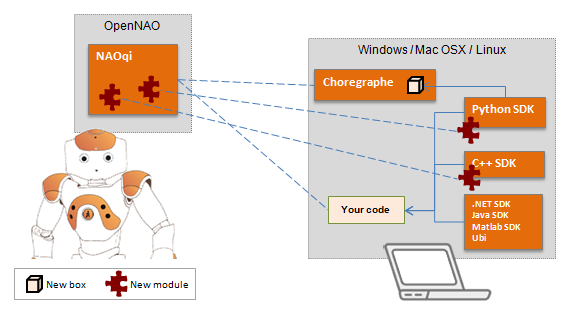
\includegraphics[scale=0.8]{Bilder/naoqi_ov.PNG}
	\caption{NAOqi Übersicht}						
	\label{f:naoqi_ov}						
\end{figure}


\subsection{Cross - Plattform/Language}

\textbf{Cross - Plattform}
\\
Cross - Plattform bedeutet Plattformunabhängigkeit gegenüber dem Betriebssystem auf dem Programmiert werden soll. Sowohl auf Linux, Windows und auf Mac kann Code für Nao programmiert werden. Allerdings kann auf Windows und Mac nur Code auf dem Computer selbst kompiliert werden, während auf Linux der Code auch auf dem Roboter selbst programmiert werden kann.
\\
\\
\textbf{Cross - Language}
\\	
Cross - Language ist nach \cite{ws:naodocu} die Eigenschaft, dass Software in C++ und in Python entwickelt werden kann. In allen Fällen, in denen die Methoden exakt gleich sind kann die \ac{API} (dt: Programmierschnittstelle), gleichgültig von welcher der unterstützten Programmiersprachen, aufgerufen werden. Die \ac{API} ist in acht Programmiersprachen verfügbar: C++, Python, .NET (C\#, Visual Basic, F\#), Java, Matlab und Urbi.

Neue NAOqi Module können nur in C++ oder Python entwickelt werden, jedoch kann die Client - API mit allen Programmiersprachen angesprochen werden. Ebenso sind nur C++ und Python auf dem Roboter unterstützt, die anderen Sprachen werden nur über \textit{Remote - Access} unterstützt. (siehe unten \textit{Proxy})
\\
\subsection{NAOqi - Prozess}
Der NAOqi - Prozess der auf dem Roboter läuft ist ein \textit{Broker} (siehe unten). Beim Start des Prozesses wird eine Konfigurationsdatei \textsf{autoload.ini} geladen, die definiert, welche Bibliotheken geladen werden sollen. Jede Bibliothek beinhaltet ein oder mehrere Module, die der Broker nutzt um deren Methoden öffentlich anzuzeigen. (siehe \ref{f:naoqi_broker1})

\begin{figure}[H]						
	\centering							
	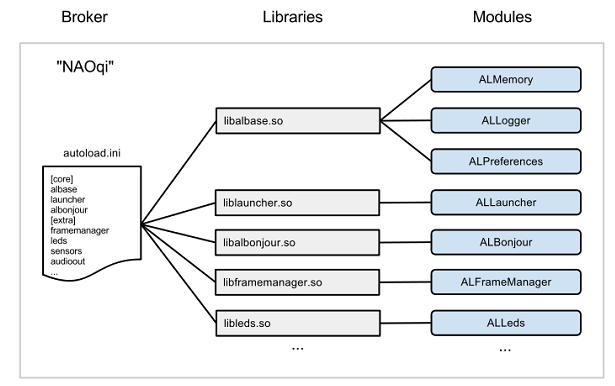
\includegraphics[scale=0.8]{Bilder/naoqi_process1.PNG}
	\caption{NAOqi Broker}						
	\label{f:naoqi_broker1}						
\end{figure}

Der Broker 	stellt einen Lookup - Service zu Verfügung, so dass jedes Modul im Baum oder verteilt im Netzwerk jede Methode finden kann, die öffentlich angezeigt wurde.

Das Laden der Module zum Start erzeugt einen Baum von Methoden, die an Module geknüpft und diese wiederum an einen Broker geknüpft sind. (siehe \ref{f:naoqi_broker2})

\begin{figure}[H]						
	\centering							
	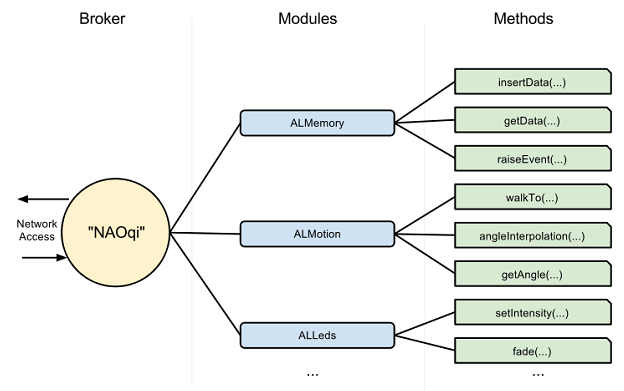
\includegraphics[scale=0.8]{Bilder/naoqi_process2.PNG}
	\caption{NAOqi Method-Tree}						
	\label{f:naoqi_broker2}						
\end{figure}
\noindent
\textbf{Broker}
\\
Der Broker ist ein Objekt, der zwei generelle Rollen einnimmt. Erstens ist das ein Verzeichnis - Dienst, mit dessen Hilfe Module und Methoden gefunden werden können und zweitens ein Netzwerk - Anschluss, der es möglich macht Methoden verknüpfter Module auch außerhalb des Prozesses aufzurufen.

Die Meiste Zeit muss sich keine Gedanken um die Broker gemacht werden, da diese ihre Arbeit selbstständig und transparent machen. Geschriebener Code kann gleich sein, ob für Aufrufe an "`remote Module"' (dt.: entfernt; anderer Prozess oder anderes System) oder "`lokale Module"' (gleicher Prozess).
\\
\\
\textbf{Proxy}
\\
Ein Proxy ist ein Stellvertreter - Objekt das sich genau so verhält, wie das Modul das es repräsentiert. Wenn ein Proxy - Objekt des ALMotion Moduls instanziiert wird, erhält das Proxy - Objekt auch alle Methoden des ALMotion Moduls.

Um ein Proxy eines Moduls zu instanziieren gibt es zwei Möglichkeiten: 
\begin{itemize}
\item Nur den Namen des Moduls benutzen. In diesem Fall muss der auszuführende Code und das Modul das verbunden werden soll im selben Broker liegen. Dies ist ein "`lokaler"' Aufruf
\item Zusätzlich zum Namen des Moduls auch die IP und den Port des Broker benutzen. In diesem Fall muss das Modul im zugehörigen Broker liegen. Dies ist ein "`remote"' Aufruf.
\end{itemize}
Der genaue Unterschied zwischen "`remote"' und "`lokalen"' Modulen wird im folgenden erklärt.
\\
\subsection{Module}
Typischerweise ist ein Modul eine Klasse innerhalb einer Bibliothek und wird automatisch instanziiert wenn diese  durch \textsf{autoload.ini} geladen wird. Neue Methoden können an Klassen gebunden werden, die von \textsf{ALModule} erben. Dadurch werden die Methoden mit ihrem Namen und ihrer Signatur dem Broker öffentlich gemacht, so dass diese anderen verfügbar wird.

Ein Modul kann, wie oben bereits erwähnt, entweder "`remote"' oder "`lokal"' sein. 

\textbf{Lokale Module } sind zwei (oder mehr) Module, die im selben Prozess gestartet wurden. Sie kommunizieren miteinander lediglich über \textbf{einen} Broker. Durch den gemeinsamen Prozess können sie sich  Variablen teilen und einander Methoden ohne Serialisierung oder Netzwerkverbindung aufrufen. Dies erlaubt die schnellste Kommunikation untereinander. Lokale Module werden als Bibliothek kompiliert und können ausschließlich auf dem Roboter ausgeführt werden. Sie sind sehr schnell und effizient im Umgang mit dem Arbeitsspeicher.

\textbf{Remote Module} kommunizieren über das Netzwerk miteinander. Jedes remote Module benötigt einen Broker um mit anderen Modulen zu sprechen. Der Broker nutzt dabei das Netzwerkprotokoll SOAP\footnote{Simple Object Access Protocol, dient u.a. dazu \textit{Remoe Procedure Calls} durchzuführen} um die Kommunikation bereitzustellen. Schnelles Ansprechen von Modulen ist über ein remote Modul nicht möglich, beispielsweise bei direkter Adressierung des Arbeitsspeichers. Remote Module werden als ausführbare Dateien kompiliert und können außerhalb des Roboters aufgerufen werden. Remote Module sind einfacher zu benutzen und können dadurch von außen einfacher debuggt werden. Allerdings sind sie langsamer und weit weniger effizient wie lokale Module. 
\\
Die Kommunikation zwischen remote Modulen kann über zwei Wege erfolgen. Erstens \textbf{Broker to Broker} und zweitens \textbf{Proxy to Broker}.
 
Der Unterschied liegt darin, dass Broker to Broker eine wechselseitige, Proxy to Broker nur eine einseitige Kommunikation eröffnet. Bei zwei Modulen B und C kann bei Broker to Broker B Methoden von C und C Methoden von B aufrufen. Bei Proxy to Broker ist dies nur in die Richtung von B nach C möglich, nicht umgekehrt. Folgendes Listing zeigt die Implementierung beider Kommunikationsarten.

\lstinputlisting
    [caption={Kommunikationsarten Module}
       \label{test},
       captionpos=b]	
 {Listings/module_comm.cs}
\noindent	
\textbf{Blocking und non - Blocking Aufrufe}
\\



\subsection{.NET SDK}
vorstellung c\# SDK, HelloWorld